\documentclass[12pt, twoside]{article}
\usepackage[francais]{babel}
\usepackage[T1]{fontenc}
\usepackage[latin1]{inputenc}
\usepackage[left=7mm, right=7mm, top=7mm, bottom=7mm]{geometry}
\usepackage{float}
\usepackage{graphicx}
\usepackage{array}
\usepackage{multirow}
\usepackage{amsmath,amssymb,mathrsfs}
\usepackage{soul}
\usepackage{textcomp}
\usepackage{eurosym}
 \usepackage{variations}
\usepackage{tabvar}


\pagestyle{empty}

\begin{document}


\section*{\center{Devoir maison 8}}


\bigskip





\fbox{

\begin{minipage}{18cm}
\textit{Devoir � rendre sur feuille grand format pour le
\textbf{vendredi 27 mai 2011}.}
\end{minipage}
}

\enskip


 \textit{Remarque: La justification et la r�daction seront compt�es dans
 le bar�me.}


\bigskip


\ul{Exercice 1}: (\textit{3 points})

\enskip



 \begin{tabular}{cc}
\begin{minipage}{14cm}
   On sait que les droites (GH) et (OU) sont parall�les et que
  AO=18cm, AH=7cm, AU=15cm et OU=9cm. 
  Calculer AG et HG. Justifier votre
  r�ponse.
   \end{minipage}
&
\qquad 
\end{tabular}


\bigskip

\medskip

\ul{Exerice 2}: (\textit{3 points})

\enskip

En utilisant les informations port�es sur la figure, calculer CG et AF.
Justifier votre r�ponse.

  



\bigskip

\bigskip

\bigskip

\bigskip


\bigskip

\bigskip

\bigskip


\bigskip

\ul{Exercice 3}: (\textit{5,5 points})

\enskip

\begin{tabular}{cc}
\begin{minipage}{13cm}
On consid�re le trap�ze DRAP tel que: (AP) soit parall�le � (DR) et � (IJ), 
AP=32mm, DR=48mm, DA=45mm, DI=15mm et
IP=5mm. 


Les points I,J et K sont align�s.

\begin{enumerate}
  \item Calculer IJ. Justifier votre r�ponse.
  \item Calculer DJ. Justifier votre r�ponse.
  \item En d�duire AJ puis calculer la valeur exacte de $\dfrac{AJ}{AD}$.
  \item Calculer JK. Justifier votre r�ponse.
\end{enumerate} 
\end{minipage}
&
\begin{minipage}{5cm}
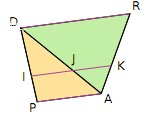
\includegraphics[width=4cm]{images/trapeze.jpg}
\end{minipage}
\end{tabular}

\bigskip

\medskip


\ul{Exercice 4}: (\textit{4 points})

\enskip

En utilisant les informations port�es sur la figure:

\begin{tabular}{cc}
\begin{minipage}{12cm}
\begin{enumerate}
  \item D�montrer que le triangle LSB est rectangle en L.
  \item Que peut-on dire des droites (LS) et (KT)? Justifier votre r�ponse.
  \item Montrer que L est le milieu de [BK]. Justifier votre r�ponse.
 \end{enumerate}
\end{minipage}
&
\begin{minipage}{6cm}
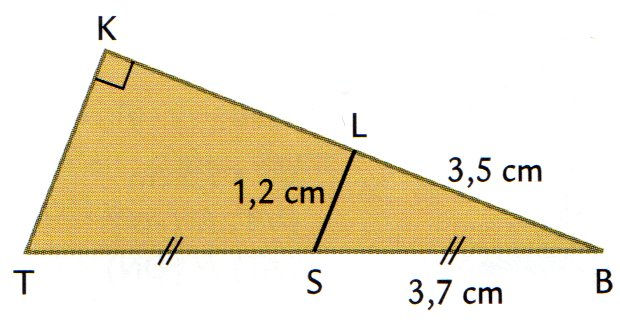
\includegraphics[width=6cm]{images/ex3.jpg}
\end{minipage}
\end{tabular}



\bigskip

\ul{Exercice 5}: (\textit{4,5 points, Extrait du brevet})

\enskip

Soit ABC un triangle tel que: AB=10,4cm , AC=9,6cm et BC=4cm.

\begin{enumerate}
  \item Faire une figure qui sera compl�t�e au fur et � mesure.
  \item D�montrer que ABC est un triangle rectangle.
  \item Soit D le point du segment [AB] tel que AD=7,8cm. Le cercle
  $\mathcal{C}$ de diam�tre [AD] recoupe le segment [AC] en E.
  
  Montrer que le triangle AED est rectangle en E. Justifier votre r�ponse.
  \item En d�duire que les droites (BC) et (DE) sont parall�les. Justifier
  votre r�ponse.
  
  \item Calculer DE. Justifier votre r�ponse.
\end{enumerate}
\end{document}
